\chapter{Materials and Software}
\label{chapter3}
After planning the report, the first week was used to introduce myself to the main components of the project. It was necessary to get used to the new software and materials so that I could find out how to use them for the required tasks.
\section{The Robot}
A Baxter robot is a programmable automaton which is already being integrated into workforces around the world \cite{baxterweb}. This robot (\textbf{\Cref{fig:baxtertorso}}) is currently very popular to use at universities as a safe robot for research purposes and this project will use the one at Leeds.
\begin{figure}[H]
    \captionsetup[figure]{justification=centering}
    \begin{subfigure}[H]{0.475\textwidth}   
        \centering 
        \caption{}
        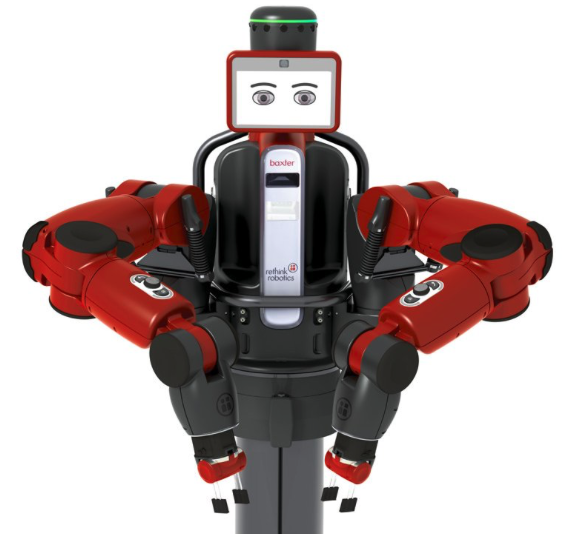
\includegraphics[width=0.75\textwidth, height=5.5cm]{baxtermain.png}
        \label{fig:baxtertorso}
    \end{subfigure}
    \begin{subfigure}[H]{0.475\textwidth}   
        \centering
        \caption{}
        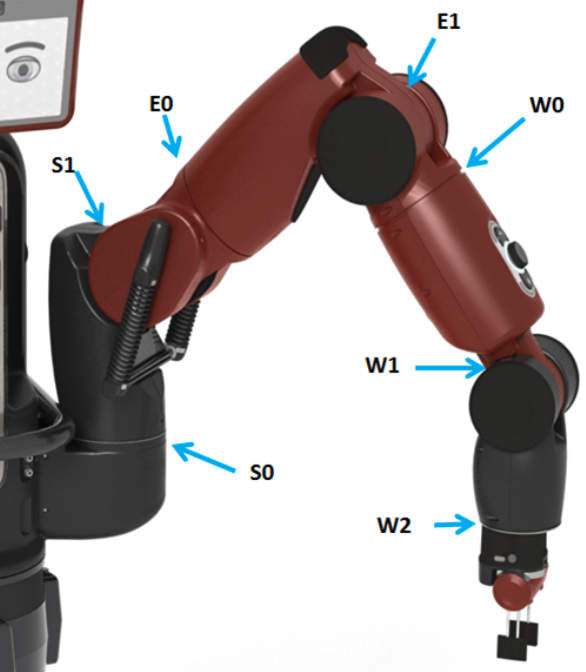
\includegraphics[width=0.55\textwidth, height=5.5cm]{baxterjoints.png}
        \label{fig:baxterjoints}
    \end{subfigure}
    \captionsetup{justification=centering}
    \caption{Baxter robot specifications. (a) Full torso of Baxter. (b) Seven labelled arm joints, present on each limb.}
\end{figure}
Baxter has three cameras to use, a right hand, a left hand and a head camera, each of which can output different resolution images for use in machine vision. He has two electronic grippers which can be customised to grip objects of different sizes, with pressure sensors to detect whether he has grabbed something. Seven joints are located on each arm (shown in \textbf{\Cref{fig:baxterjoints}}), with humanoid movement, which can be controlled by specifying specific joint positions or torques at each joint.
\section{Kinect}
The Kinect has two cameras, used to detect objects with depth detection. It has been utilised in many areas of robotics as a more accurate vision method, creating 3D objects by looking at the Kinect's pointcloud, an array of points with an x, y and z coordinate, containing RGB values for each one. The Kinect in the robotics department was set up to work with Baxter. It was calibrated with a rectangular checkerboard to set up the Kinect drivers, which could then set up the ROS transform (explained in \textbf{\Cref{ssec:fft}} below) between Baxter and the Kinect. Baxter could then know his own coordinate system with respect to the Kinect.
\section{Software}
There were multiple pieces of software that I had not used before, so some research needed to be done into them. The most helpful tutorials and files on most of the software were located in their respective online documentation.
\subsection{OpenCV}
OpenCV is a very useful open source implementation of vision techniques and functions. Having not used OpenCV before, I decided to write the OpenCV code in this project in Python (as there is a C++ and Python version of the module). It was very easy to pickup from the documentation and tutorials and most of the features were well explained online. It is written in an optimized C/C++ library, which turned out to be very quick and efficient to use on image analysis, even from Baxter's camera video feeds outputting high resolution images.
\subsection{PCL Library}
The PCL library is a C++ library which is open source and written in C++. It allows you to process and analyse pointclouds. It is rather poorly documented and there weren't many examples to find online so it was very much a trial and error to learn the functions and processes in this library. One of the main problems is it required a lot of manual manipulation and conversions of pointcloud types. There were multiple types of pointcloud data such as PointCloudXYZ, PointCloud2 or PointCloudXYZRGB, which would have to be converted and switched between depending on the function you wanted to use. Manual manipulation of pointclouds was also difficult, as you needed to use C++ boost iterators to access the indices of the points before then implementing the custom algorithms over the whole cloud.
\section{ROS}
ROS (or robot operating system) is a very interesting piece of software that is open-source and very widely used to program robots. It is a very useful, adaptable piece of software that is written using it's main features of nodes and topics. Nodes are pieces of code that can be constantly run in a terminal window and be in contact with other nodes. Topics are custom data items that are constantly published as information from Baxter to the terminal. ROS nodes can access these topics to get information from Baxter or send information to him. Custom topics can be created and published via ROS to publish custom information between nodes.
\newline\newline
For example, in Baxter's vision system for the shop, Baxter uses his right hand camera to view the sweets on the table. To carry out the structure of this task in ROS, a sweet vision node is created. That node would accept the right hand camera image topic to retrieve the sweet image to analyse. Then, after analysing the image, the node would then publish a list of the sweet locations on a custom topic, with a different node receiving those positions, so Baxter knew where to pick them up.
\subsection{RViz}
RViz is a very useful ROS package that was used in almost every aspect of the project. It can be used to visualise the many topics within ROS. The idea of RViz is that if any information is published as a topic, then RViz should be able to access and display that information in real-time. Baxter's robot model can be imported into the software and it's movements will be constantly updated, as shown below in \textbf{\Cref{fig:rvizscreen}}.
\begin{figure}[H]
        \centering 
        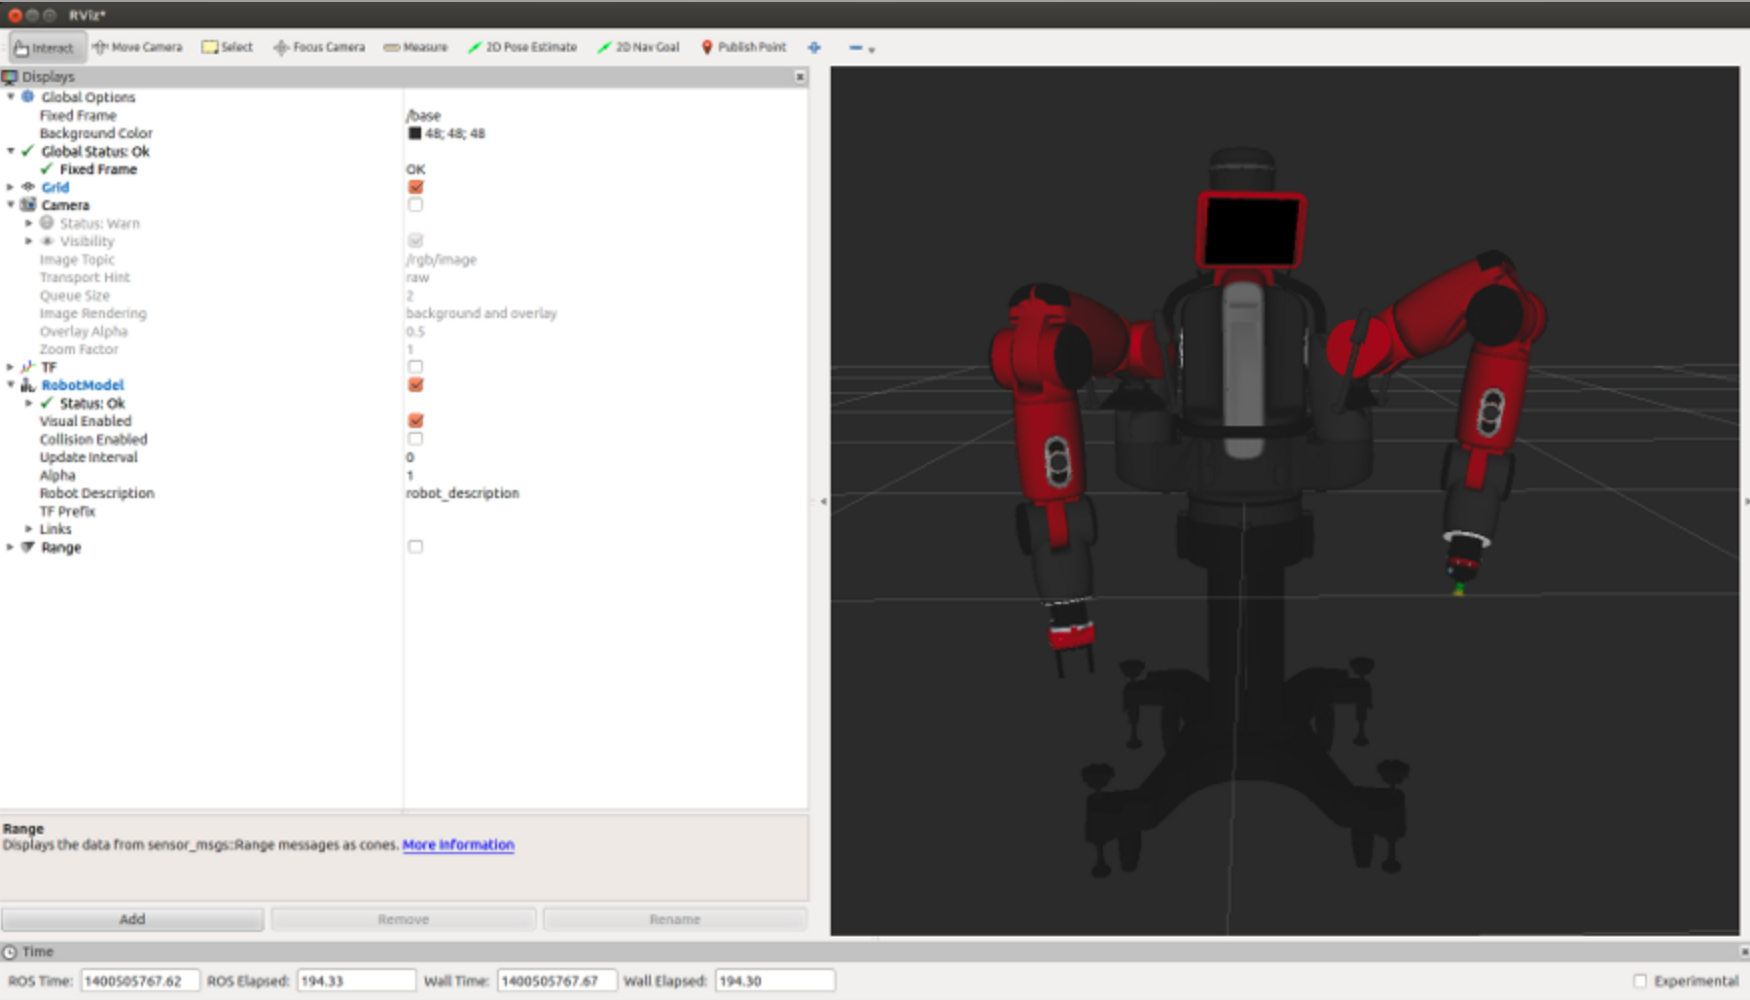
\includegraphics[width=0.7\textwidth, height=7cm]{rvizscreen.png}
        \caption{Baxter's model imported into RViz.}
        \label{fig:rvizscreen}
\end{figure} 
From the left hand toolbar, a multitude of extra visualisations can be added to view alongside Baxter: the Kinect's depthcloud, axes transforms for any fixed frame and more. Throughout the project, if a vision system needed to detect something, RViz could be used to make sure it was correctly aligned with Baxter and the Kinect. This technique was used and can be seen many times in the Methods section of the report.
\subsection{Fixed Frame Transforms}
\label{ssec:fft}
A key aspect of creating the integrated movement system was understanding the concept of fixed frames and transforms. In ROS, Baxter contains information for multiple transforms between every joint and sections of his body. These are known at all times to help know where a point is relative to one part, say the hand, against Baxter's torso. This method works similarly for the Kinect, where Baxter's torso coordinate system, is linked to the Kinect's coordinate system via a transform, which can be accessed by certain methods within ROS.
\begin{figure}[H]
        \centering 
        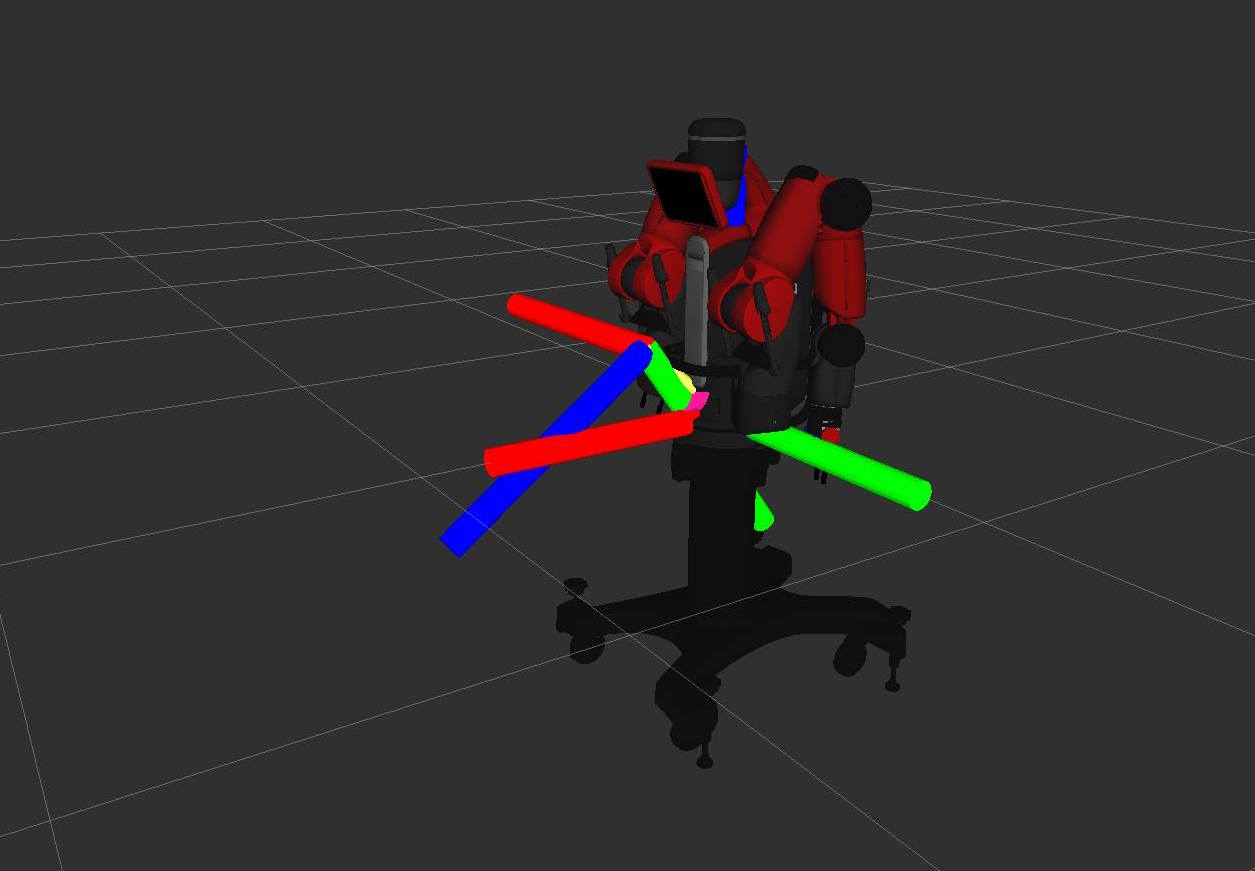
\includegraphics[width=0.475\textwidth, height=5cm]{fixedframe.jpg}
        \caption{Image showing axes transforms between the Kinect and Baxter's torso frame, with the red, green and blue lines representing the x, y and z axes respectively.}
        \label{fig:fixedframe}
\end{figure}
Fixed coordinate systems were constantly used in testing the vision systems in this project, mainly within RViz. Everytime a coordinate or shape was recognised within the vision system, they could be published to RViz using a PointStamped object, which can be published in a particular coordinate system. Therefore, by publishing in one frame, transforming then publishing it another, RViz can show whether a point is correctly detected and whether it is in the correct frame or not.
\newline\newline
This principle was used in the bowl recognition system, where after the centre of the bowl was obtained, Baxter needed to know where the centre of the bowl was in it's main torso coordinate system before a movement command could be made. The system then looked up the transform between the Kinect and Baxter's torso to transform the 3D coordinate between coordinate systems. In \textbf{\Cref{fig:fixedframe}}, RViz shows the axes for the Kinect's frame and Baxter's torso frame.
\subsection{Custom Service Requests}
\label{ssec:customsrv}
The idea that Baxter's movements would all be based on the current states of his vision system - depending upon where both the sweets and the bowl were, meant there needed to be a method developed for Baxter's movement system to request information from the vision system. This was implemented via Services, which is a technique in ROS that allows a custom message to be sent, and then received between two nodes.
\newline\newline
Custom services were extremely useful as a method to send information back and forth between the nodes, which needed to be utilised a lot when integrating the whole ROS system together. Whilst I had implemented and coded multiple nodes for each aspect of the system, they only worked on their own. Without one main node being able to retrieve all of the information for each system, the system wouldn't be able to work together. For example, a custom service request is shown and explained below.
\begin{lstlisting}

string reset
...
float[] sweetPositions
\end{lstlisting}
\vspace{0.5cm}
This request was stored in a .srv file and was used in the shop's integrated system. The main shop node uses this service file as a request by first, publishing the service on a new node and sends a 'string reset' item within that request. Then, the sweet vision system has a constant client listening out for this service message and then, when it received it, it calculated the current sweet positions and sent back the message with those positions stored in the 'float[] sweetPositions'. Then the main shop node can receive and process these positions. As you can see, this approach came in very handy and was used quite often for the main node to retrieve information for the shop.
\section{Github Repository}
All of the code files mentioned throughout the upcoming chapters of the report are stored within the src folder of the Github repository, so they can be cloned directly into a created ROS workspace. The src directory is divided into multiple catkin packages - perception, interaction and manipulation to make the files easier to navigate. There is a testing and videos folder, providing evidence for the testing and data collected. Finally, there is a report folder, containing multiple draft versions of the report during it's development, from the initial version 0 to the final draft. Overall, the repository has been well maintained and the commit messages are self explanatory in terms of their purpose.
